\section{Conclusions}





\section{Future Work}

More immediate work ought to be done to further validate the proposed ADCBC method from \chap{ch:delay-bcs}, including investigating the interpolation of $\cl{L}_{1/5}$ values and ensuring that acoustic energy does not trivially increase over long time periods without a flame. Having said that, the method provides a framework for multiple different thermoacoustic applications, particularly for those taking place in long tubes. Thermodiffusive and thermoacoustically unstable flames can already be modelled with the caveat that the rapidly changing flame speeds of thermodiffusive flames likely mean it will exit the DNS domain. To remedy this, dynamic inflow velocities are required which do not couple to the acoustics and counteract the mean flame speed. This is also useful for other, non-thermodiffusive flames which reach secondary instability since the flame speed changes drastically under this regime. Another typical test case and one which is used to test the D-TDIBC method in \cite{douasbin2018DelayedtimeDomainImpedance} is a flame in a strong counterflow, held in place by an adiabatic cylindrical flame holder. Comparisons to their calculated eigenmodes could be found by simulating the same model geometry whilst also providing mode shapes in the fictitious domain. Furthermore, ADCBC should also be easily applicable to flames passing through arrays of cylinders (or other porous geometries). Typically, this is expensive to model due to the task of fitting the discretisation to the complex body and the large scale disparity in thermoacoustics. Utilising the LABFM discretisation in the SUNSET code coupled to low-order ADCBC allows us to model this phenomena for the cost of discretising only the flame and its surrounding hydrodynamic region.

Furthermore, the use of characteristic boundaries allows us to freely impose incoming acoustics through the inflow, $\cl{L}_{5, \rm{imposed}}(t)$ and outflow, $\cl{L}_{1, \rm{imposed}}(t)$ on top of their existing values from the acoustic delay. By implementing an imposed e.g. sinusoidal forcing to model an upstream loudspeaker playing a pure tone, we can trigger secondary instabilities in a model version of \cite{searby1991ParametricAcousticInstability}. This would allow us to more efficiently investigate secondary instability modes and their flame structures. This could be potentially elaborated into three dimensions to try and recreate the wavenumber measurements of \cite{delfin2024DeterminationMethodMarkstein}. Turbulent flow can also be imposed through the VFCBC method established in \cite{guezennec2009AcousticallyNonreflectingReflecting} and an attempt could be made to implement this on top of the existing ADCBC method, as above. Turbulent characteristic outflows would also need to be implemented for compatibility. This may allow us to simulate faster flows in broader domains which are expected to be turbulent, as well as potentially allowing us to observe the self-turbulent flames seen resulting from secondary instability in \cite{searby1992AcousticInstabilityPremixed}. Thus far, we have gotten away with values of $\abs{R_{\rm{U}/\rm{D}}} = 1$, but more realistic boundaries have impedances which vary with frequency. Could this be explored using some sort of spectral filtering on delayed $\cl{L}_{1/5}$ values? Practically speaking, a low-pass filter could be used to remove high-frequency noise and improve the quality of observed low frequency modes (at the cost of precluding high-frequency ones). More generally, the non-linear acoustic effects which are not being modelled here could be included by couple an acoustic solver to the DNS inflow and outflow. Using for example a boundary element method or analytical techniques, acoustics around some up- or downstream geometry can be solved in tandem with the DNS domain. This could enable us to simulate a flame tube with a porous plug and compare to the analysis of \cite{gaton-perez2025MitigationThermoacousticInstabilities}.



\section{Planning}

% 9 quarters left ...

% Stuff in plan-Y3.md basically


\begin{figure}[t]
\centering
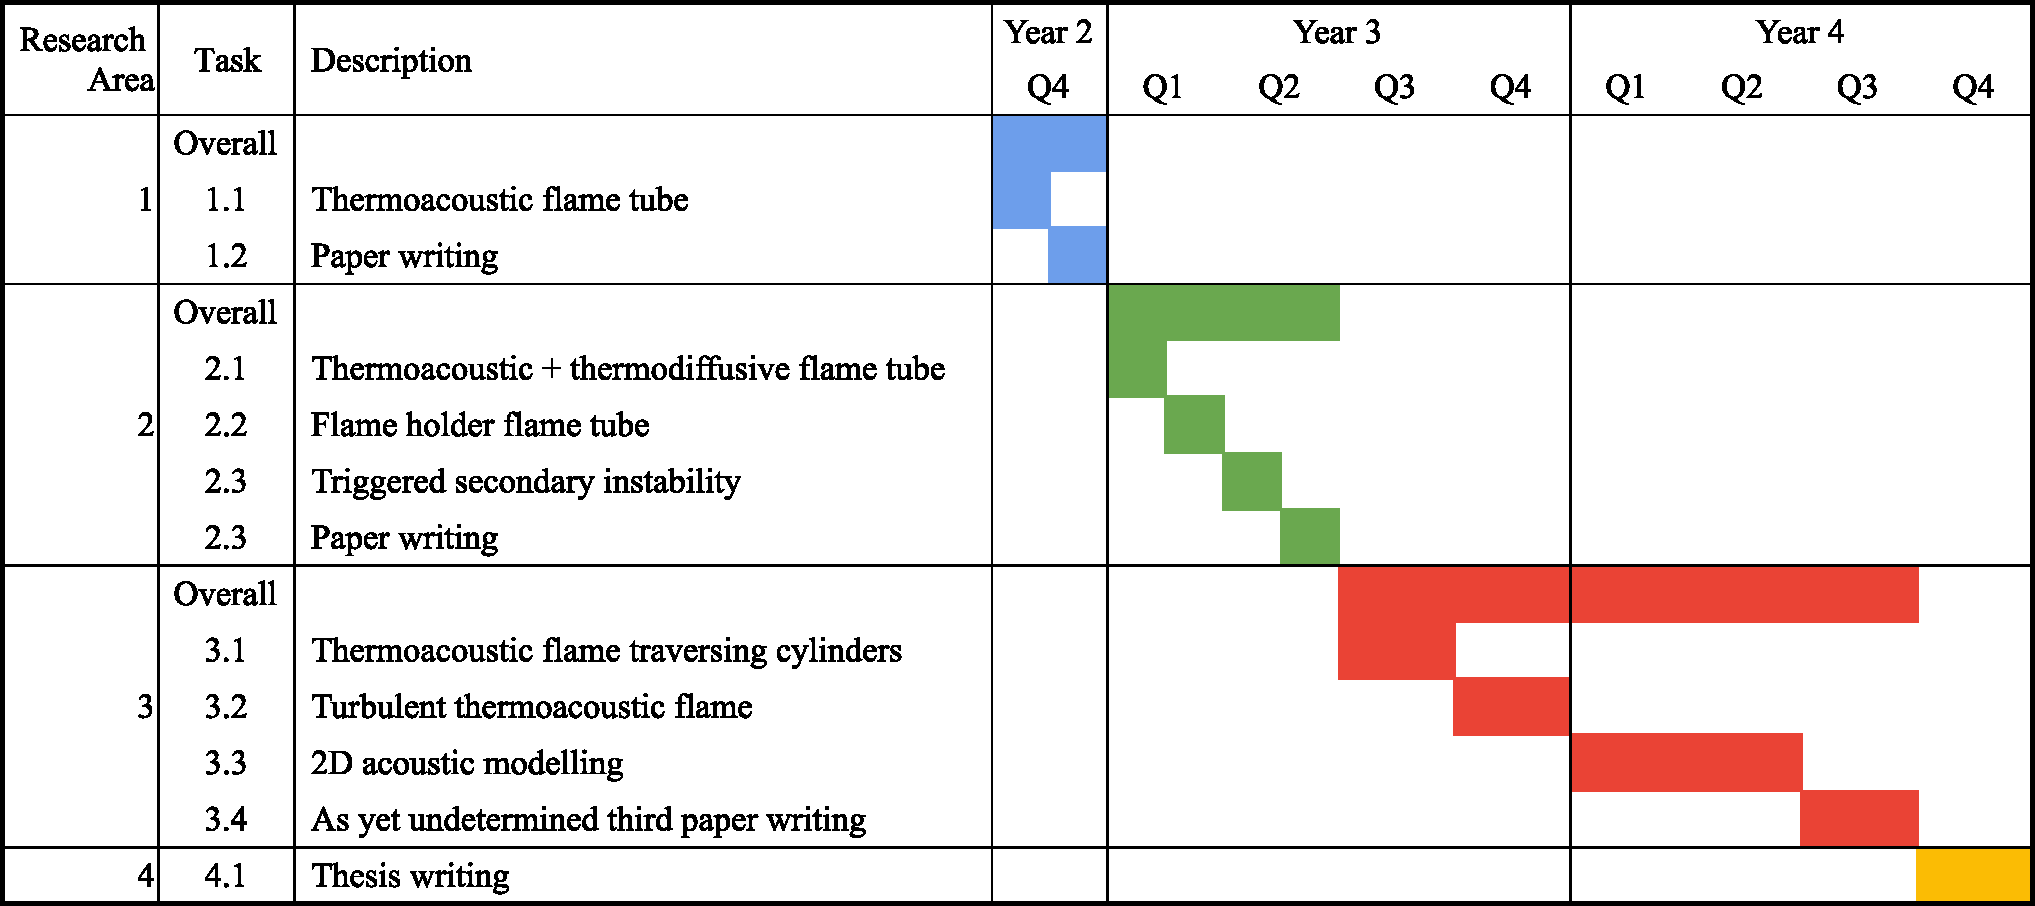
\includegraphics[scale=0.5]{assets/graphs/2YR_Gantt.pdf}
\caption{Gantt chart!}
\label{fig:gantt}
\end{figure}

